\section{Data generation}

The test data is generated around a manually chosen ground truth model (line or circle).
I've generated the following data set for testing:
\begin{itemize}
  \item As there's 4 different inlier ratios, and 4 different thresholds, I've
    created 16 different data sets per model.
  \item Each sets holds 200 data points in the range of x = [-50, 50].
  \item The given ratio of data points is inside the given threshold. The rest
    are scattered randomly.
  \item The circle and line models (naturally) use different test data sets, so
    there's 32 data sets in total. The different algorithms use the same data.
\end{itemize}

\section{Testing procedure}

I've implemented the RANSAC algorithm for the line and circle models. I've also
implemented the bonus algorithms R-RANSAC and MSAC, both for line and circle
approximation. Each of these algorithms is run 16 times; Once for each dataset.

\section{Effect of parameters on RANSAC performance}

The parameters we are varying are the ratio of inliers in the dataset, and the
inlier ratio.

The ratio of inliers seems to be have the biggest effect on processing time and
performance, mostly because it has a big effect on the number of iterations.
The higher the ratio, the less iterations there are, which is of course faster,
but also way more unstable. For example, with a ratio of 90\% inliers, there's
only 5 iterations. In this case, RANSAC approximation can be very bad. The mean
squared error of these approximated models compared to the ground truth can
easily be in the hundreds (>100).

RANSAC functions worse than usual on all the 90\% inlier data sets. This seems
counter-intuitive, considering that in the data set in question, the points are
located most closely to the ground truth model. However, we have to remember
that because the high percent of inliers, the iteration count is also the
lowest.

In figure~\ref{fig:circles_RANSAC} we have a set of plots of approximated
RANSAC circle models, with the data set the models are computed on. As
mentioned before, the approximated models seem to be worst on the 90\% inlier
data sets. Even though the data is arranged clearly, we have a big chance of
sampling bad points, resulting in a bad approximation.

\begin{figure}[H]
  \centering
  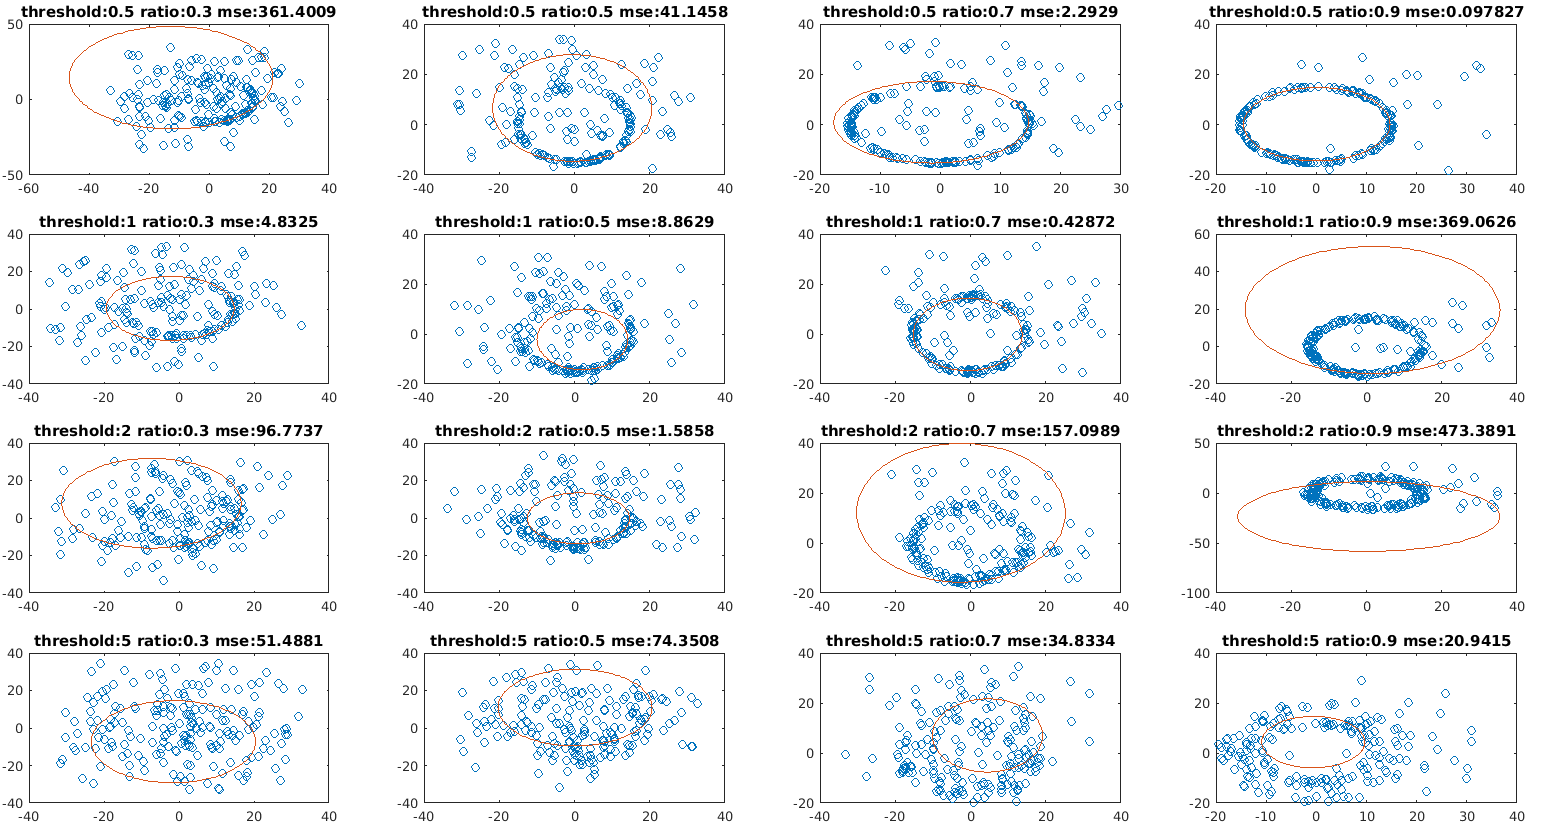
\includegraphics[width=1\linewidth]{circles_RANSAC}
  \caption{RANSAC approximated circle models, with different data sets.}\label{fig:circles_RANSAC}
\end{figure}

Although the data sets with 30\% of inliers have a lot of iterations, ie.\
chances to get a good model, the data is simply a lot more scattered and harder
to work with, leading to subpar models. However, they still seem to be better
than the 90\% inlier models. The best performing models seem to be the ones
using the 50\% and 70\% inlier data sets. Apparently they hit a sweet spot
where the data is good enough for approximation, while still doing enough
iterations to have a chance of finding a good model.

\section{Processing time vs.\ performance}

Just from using the iteration function \( N = \frac{\log(1-p)}{\log(1-r^s)} \),
we can see that increasing the probability p of having at least inlier, the
number of iterations to be calculated increases. If we make a plot
p-N~\ref{fig:performance-plot}, we see
that the number of iterations increases exponentially at around the 90\%
probability mark. So if we want to optimize between computation performance and
RANSAC accuracy, the 90\% probability of finding an inlier seems to be optimal.

\begin{figure}[H]
  \centering
  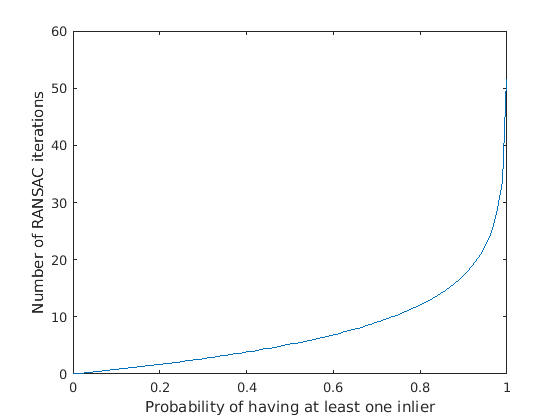
\includegraphics[width=0.8\linewidth]{performance-plot}
  \caption{Plot of the iteration count function, with sample size 3, and an
  inlier ratio of 50\%.}\label{fig:performance-plot}
\end{figure}

\section{Problems with RANSAC}

The main problem with RANSAC is its iterative and random nature; It's not
guaranteed to find an optimal, or even a good solution. That is why it's
important to ensure that the number of iterations is enough to find a workable
solution. It's also not a deterministic algorithm, which is obvious considering
the random sampling.  It can also be difficult to find good threshold and
probability parameters for a specific problem.

\section{Comparison of the RANSAC algorithms}

Comparing running times, R-RANSAC is clearly faster than both RANSAC and MSAC\@.
Taking an average of \(>10\) runs, R-RANSAC takes usually 0.06s, RANSAC 0.14s and
MSAC 0.13s. As can be seen, maybe surprisingly MSAC performs slightly faster
than vanilla RANSAC\@. In general, all algorithms seemed to be very stable in
their runtimes.

R-RANSAC is however a lot less accurate. Especially in situations, where there
aren't any good models to find, R-RANSAC can discard the tolerable ones,
leaving it only with the worst models. If we calculate the mean squared error
of the different algorithms in relation to the ground truth model, R-RANSAC has
an error value of over 3 times that of vanilla RANSAC\@. This is intuitive,
because R-RANSAC introduces further random elements in the pre-evaluation
stage.

MSAC performs overall slightly better than RANSAC, but it seems to be
especially performant in data sets with a low number of inliers, ie.\ the 30\%
inlier set, where it results in much better models than vanilla RANSAC\@.







